
\subsection{Client}
Die client is het deel van Canvas.hs dat in de browser van de gebruiker draait. Het voornaamste onderdeel van de client is het canvaselement waarin de output getekend wordt door KineticJS. Daarboven zit de Canvas.hs JavaScript-applicatie die de verbinding onderhoudt met de module en de relevante output aan KineticJS doorgeeft om te tekenen.

\autoref{fig:architecture_client} illustreert de architectuur van de client. Deze is opgebouwd uit een webpagina die via HTTP van de server wordt geladen. Deze webpagina bevat onder andere de benodigde bestanden voor de JavaScript-applicatie en het canvas waarop getekend zal worden. Verder bevat de client de JavaScript-applicatie zelf, deze wordt, samen met de belangrijkste ontwerpbeslissingen voor deze applicatie, hieronder besproken.

\begin{figure}
\begin{center}
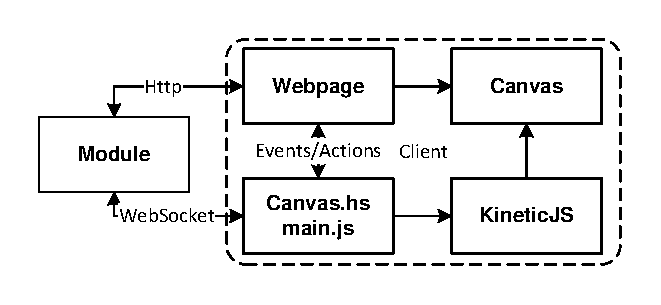
\includegraphics[keepaspectratio,width=\textwidth]{./images/client_architecture.pdf}
\caption{Architectuur van de client}
\label{fig:architecture_client}
\end{center}
\end{figure}

\subsubsection{Canvas/Events}
Vanuit de module ontvangt de JavaScript-applicatie via de WebSocketverbinding Output. Deze output wordt opgedeeld in acties en een te tekenen grafische boom. Deze boom wordt omgezet in de structuur van KineticJS. Voor de shapes uit de boom waarvan aangegeven is dat ze ge\"interesseerd zijn in events worden eventlisteners toegevoegd. Wanneer de volledige structuur opgebouwd is wordt de oude structuur weggegooid en de nieuwe structuur op het canvas getekend. Een uitgebreid overzicht van alle shapes, acties en events kan gevonden worden in \autoref{sec:gebruikershandleiding}: de gebruikershandleiding.

\paragraph{Mousedrag}
Standaard ondersteunt KineticJS mousedrag events, maar door de manier waarop Canvas.hs iedere keer opnieuw de output genereert raken de events van KineticJS verloren. Daarom maakt Canvas.hs gebruik van een eigen implementatie van mousedrag in de Canvas. Een mousedrag begint met een MouseDownEvent. Vanaf dat moment houdt de JavaScript-applicatie een ID bij van het huidige element. Alle opvolgende MouseMoveEvents zijn drag events die naar de client worden verstuurd. Deze MouseMoveEvents worden doorgegeven naar de Canvas.hs module met de vorige coördinaten van de muis en de huidige coördinaten van de muis.
Op deze manier kan de module bepalen wat er moet gebeuren tijdens het draggen. Op het moment dat het programma aangeeft niet meer ge\"interesseerd te zijn in drag events op dat ID of in het geval van een MouseUpEvent stopt de drag in de client.

\subsubsection{Acties}
Vanuit de Canvas.hs module kunnen er een aantal acties verzonden worden naar de JavaScript-applicatie. Dit kunnen acties zijn als het openen van de Debug-console (zie \autoref{par:debugconsole}) of het downloaden van een bestand. De state van deze acties, bijvoorbeeld of de debug console geopend of gesloten is, wordt bijgehouden in de JavaScript-applicatie zelf.

\paragraph{Browserrestricties}
Canvas.hs biedt de optie om de canvas in volledigscherm te laten weergeven. Door veiligheidsfunctionaliteiten in de huidige webbrowsers is het niet mogelijk om direct naar volledigscherm te gaan met behulp van JavaScript. Dit is alleen mogelijk vanuit klik- en toetsenbordevents. Daarom krijgt de gebruiker eerst een menu te zien voordat de browser naar volledigscherm gaat. Dezelfde veiligheidsrestricties zijn er voor het bestandenselectiemenu, hierdoor heeft Canvas.hs daar ook een menu voor.

\paragraph{Debug Console} \label{par:debugconsole}
Voor de programmeur die gebruik gaat maken van de Canvas.hs library is het belangrijk dat zijn interface er zo uit ziet zoals hij dit wil. Ongetwijfeld zal een programmeur tegen problemen aanlopen bij het bouwen van de interface die hij niet had voorzien bij het schrijven van zijn code. Om probleemoplossing hiervan te vergemakkelijken bevat Canvas.hs een debug console waarin alle getekende shapes tekstueel inzichtelijk worden gemaakt. Door middel van de \inlinecode{Debug-Action} is het mogelijk om vanuit de user application de debug console te tonen of te verbergen.